\section{Thermalization via a Nonlinear Boson Diffusion Equation (NBDE)}

\begin{frame}{Deriving the Nonlinear Boson Diffusion Equation I}
\vspace{0.5em}
The following derivation follows reference \cite{Wolschin2018}. \\[0.5em]
\begin{itemize}
\item The starting point for our investigation is the \alert{Boltzmann eqn.} (cf. Pavel's talk). %write it down
\item For \alert{spatial homogeneity} of the the boson distribution function $f(\mathbf{x}, \mathbf{p}, t)$ and a \alert{spherically symmetric momentum dependence} the equation for the single-particle occupation numbers  $n_j \equiv n_{\mathrm{th}}(\varepsilon_j,t)$ reads:
\begin{align}
\frac{\partial n_1}{\partial t} &= \sum_{\varepsilon_2,\varepsilon_3,\varepsilon_4}\langle V^{\phantom{.}2}\rangle G(\varepsilon_1+\varepsilon_2,\varepsilon_3+\varepsilon_4)\\
&\times \left[(1+n_1)(1+n_2)n_3n_4 - (1+n_3)(1+n_4)n_1n_2\right]
\end{align}

\item The \alert{collision term} can be written in the form of a \alert{Master eqn.}:
\begin{equation}
\frac{\partial n_1}{\partial_t} = (1+n_1)\sum_{\varepsilon_4}W_{4\rightarrow 1}n_4	- \sum_{\varepsilon_4}W_{1\rightarrow 4}(1+n_4)	
\end{equation}
with
\begin{equation}
W_{4\rightarrow 1}=  W_{41}g_1 = \sum_{\varepsilon_2, \varepsilon_3} \langle V^{\phantom{.}2}\rangle G(\varepsilon_1+\varepsilon_2,\varepsilon_3+\varepsilon_4)(1+n_2)n_3
\end{equation}
\end{itemize} 
\end{frame}

\begin{frame}{Deriving the Nonlinear Boson Diffusion Equation II}
\begin{itemize}
	\item In continuum $\sum\rightarrow\int$ and introduce \alert{density of states} $g_j \equiv g(\varepsilon_j)$.
	\item If $G$ acquires a width in a finite system: 
	\begin{equation}
		W_{14}=W_{41}=W\left[\frac{1}{2}(\varepsilon_4+\varepsilon_1),\underbrace{\abs{\varepsilon_4-\varepsilon_1}}_{=: x}\right]
	\end{equation}
	\item Perform a \alert{gradient expansion} of $n_4$ and $g_4n_4$ around $x\approx 0$.
	\item Introduce \alert{transport coefficients} via moments of the transition probability:
\begin{align}
	D &= \frac{g_1}{2}\int\limits_0^{\infty}\dd x\ W(\varepsilon_1,x) \ x^2 \\
	v &= g_1^{-1}\frac{d}{d\varepsilon_1}(g_1D) 
\end{align}
\end{itemize}
\end{frame}


\begin{frame}{Deriving the Nonlinear Boson Diffusion Equation III}
\begin{itemize}
	\item Nonlinear partial differential equation for $n \equiv n(\varepsilon_1,t) = n(\varepsilon,t)$:
		\begin{equation}
			\frac{\partial n}{\partial t} = -\frac{\partial}{\partial\varepsilon}\left[v\cdot n(1+n) + n\frac{\partial n}{\partial\varepsilon}\right] + \frac{\partial^2}{\partial\varepsilon^2}\left[Dn\right]\label{eqn:nbde1}
		\end{equation}

	\item Consider the limit of constant transport coefficients:
		\begin{equation}
			\frac{\partial n}{\partial t} = -v\frac{\partial}{\partial\varepsilon}\left[n(1+n)\right] + D\frac{\partial^2 n}{\partial\varepsilon^2}\label{eqn:nbde2}
		\end{equation}

\item Thermal \alert{Bose-Einstein distribution} provides stationary solution:
\begin{equation}
	n_{\mathrm{eq}}(\varepsilon) = \frac{1}{\exp(\frac{\varepsilon-\mu}{T}) - 1}
\end{equation}
\end{itemize}
\end{frame}

\begin{frame}{Some Remarks}
\begin{itemize}
	\item The present model does \alert{not} resolve the 2nd-order phase transition.
	\item The effects of condensation are included (cf. the following figures).
	\item A treatment resolving the singularity at $\epsilon=\mu$ is presented later.
\end{itemize}
\end{frame}

\begin{frame}{Linear Relaxation-Time Approximation (RTA)}
\begin{itemize}
	\item Given some initial distribution $n_{\mathrm{i}}(\varepsilon)$ we find an approximated solution for the thermalization process via the RTA:
\begin{equation}
	\frac{\partial n_{\mathrm{rel}}}{\partial t} = \frac{(n_{\mathrm{eq}} - n_{\mathrm{
rel}})}{\tau_{\mathrm{eq}}}
\end{equation}
with solution:
\begin{equation}
	n_{\mathrm{rel}}(\varepsilon,t) = n_{\mathrm{i}}(\varepsilon)\cdot\exp\left(-\frac{t}{\tau_{\mathrm{eq}}}\right) +  n_{\mathrm{eq}}(\varepsilon)\left(1-\exp\left(-\frac{t}{\tau_{\mathrm{eq}}}\right)\right)
\end{equation}	
where $\tau_{\mathrm{eq}} = 4D/(9v^2)$.
\item Motivated by the study of early stages of RHICs, the initial distribution is chosen such that:
\begin{equation}
	n_{\mathrm{i}}(\varepsilon) = N_{\mathrm{i}}\cdot\theta\left(1-\varepsilon/Q_{\mathrm{s}}\right)\cdot\theta(\varepsilon) \label{eqn:rta_initial}
\end{equation}
with limiting momentum $Q_{\mathrm{s}} \sim \tau_0^{-1} \approx 1\ \mathrm{GeV}$.\mycite{Mueller1999}
\end{itemize}
\end{frame}

\begin{frame}{Results for the RTA}
\begin{figure}[H]
\centering
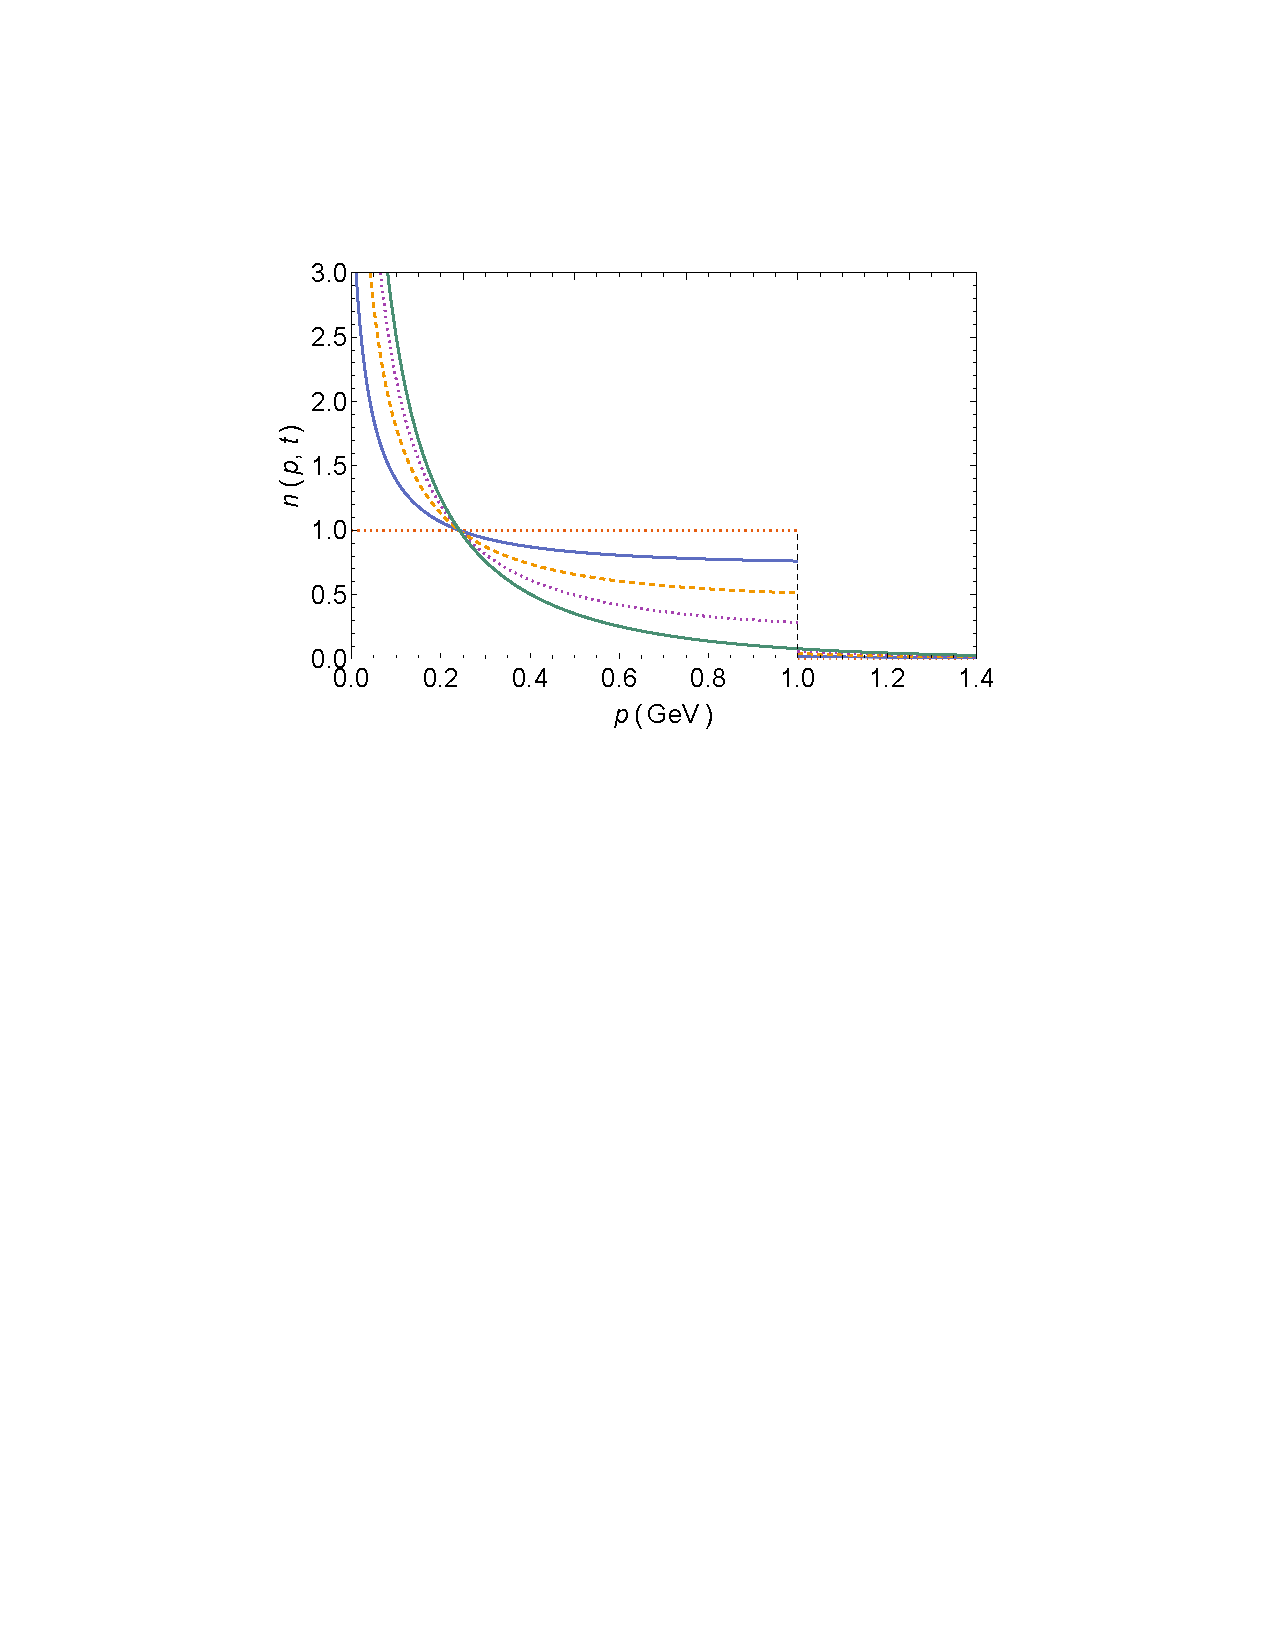
\includegraphics[width=0.8\textwidth]{figures/rta}
\caption{Relaxation of a finite Bose system towards the equilibrium. \cite{Wolschin2018} \\ 
Here $T = -D/v \simeq 0.4\ \mathrm{GeV}$, $\tau_{\mathrm{eq}} = 4D/(9v^2) = 0.33\cdot 10^{-23} \mathrm{s} \simeq 1\ \mathrm{fm/c}$ and the timesteps are $\left\{0.1, 0.25, 0.5,\infty\right\}$ (in units of $10^{-23}s$) from top to bottom.}
\end{figure}
\end{frame}
%TODO: Maybe add another slide about conservation etc.

\begin{frame}{Exact Solution of the Nonlinear Boson Diffusion Equation} 
\begin{itemize}
	\item To solve eqn. (\ref{eqn:nbde1}) analytically, we perform the following \alert{nonlinear transformation:}
	\begin{equation}
		n(\varepsilon,t) = -\frac{D}{v}\frac{\partial \ln \mathcal{Z}(\varepsilon,t)}{\partial\varepsilon}
	\end{equation}
	which reduces our problem to a \alert{linear diffusion eqn.} for $ \mathcal{Z}(\varepsilon,t)$:
	\begin{equation}
		\frac{\partial  \mathcal{Z}}{\partial t} = -v\frac{\partial  \mathcal{Z}}{\partial \varepsilon} +  D\frac{\partial^2  \mathcal{Z}}{\partial \varepsilon^2}
	\end{equation}
	\item Solutions to this equation can be written as:
 \begin{equation}
n(\varepsilon, t)=\frac{1}{2 v} \frac{\int_{-\infty}^{+\infty} \frac{\varepsilon-x}{t} F(x)\cdot G_{\mathrm{free}}(\varepsilon-x,t)\ \dd x}{\int_{-\infty}^{+\infty} F(x)\cdot G_{\mathrm{free}}(\varepsilon-x,t)\ \dd x}-\frac{1}{2}
\end{equation}
\end{itemize}
\end{frame}

\begin{frame}{Additional Definitions} 
\begin{itemize}
\item The quantities appearing in the solution are the \alert{free Green's function}
\begin{align}
	G_{\mathrm{free}}(\varepsilon-x,t) = \exp\left[-\frac{(\varepsilon-x)^2}{4Dt}\right],\\
\end{align}
and the implementation of the \alert{initial conditions}
\begin{equation}
	    F(x)  = \exp\left[-\frac{1}{2D}(vx+2v\int_0^x n_{\mathrm{i}}(y) \dd y) \right].
\end{equation}
\item They define the \alert{free partition function} via: 
\begin{equation}
	\mathcal{Z}(\varepsilon,t) = a(t)\cdot\int_{\infty}^{\infty} G_{\mathrm{free}}(\varepsilon,x,t)\cdot F(x)\ \dd x
\end{equation}
\end{itemize}
\end{frame}


\begin{frame}{Results for the Solution of the NBDE I}
\begin{figure}[H]
\centering
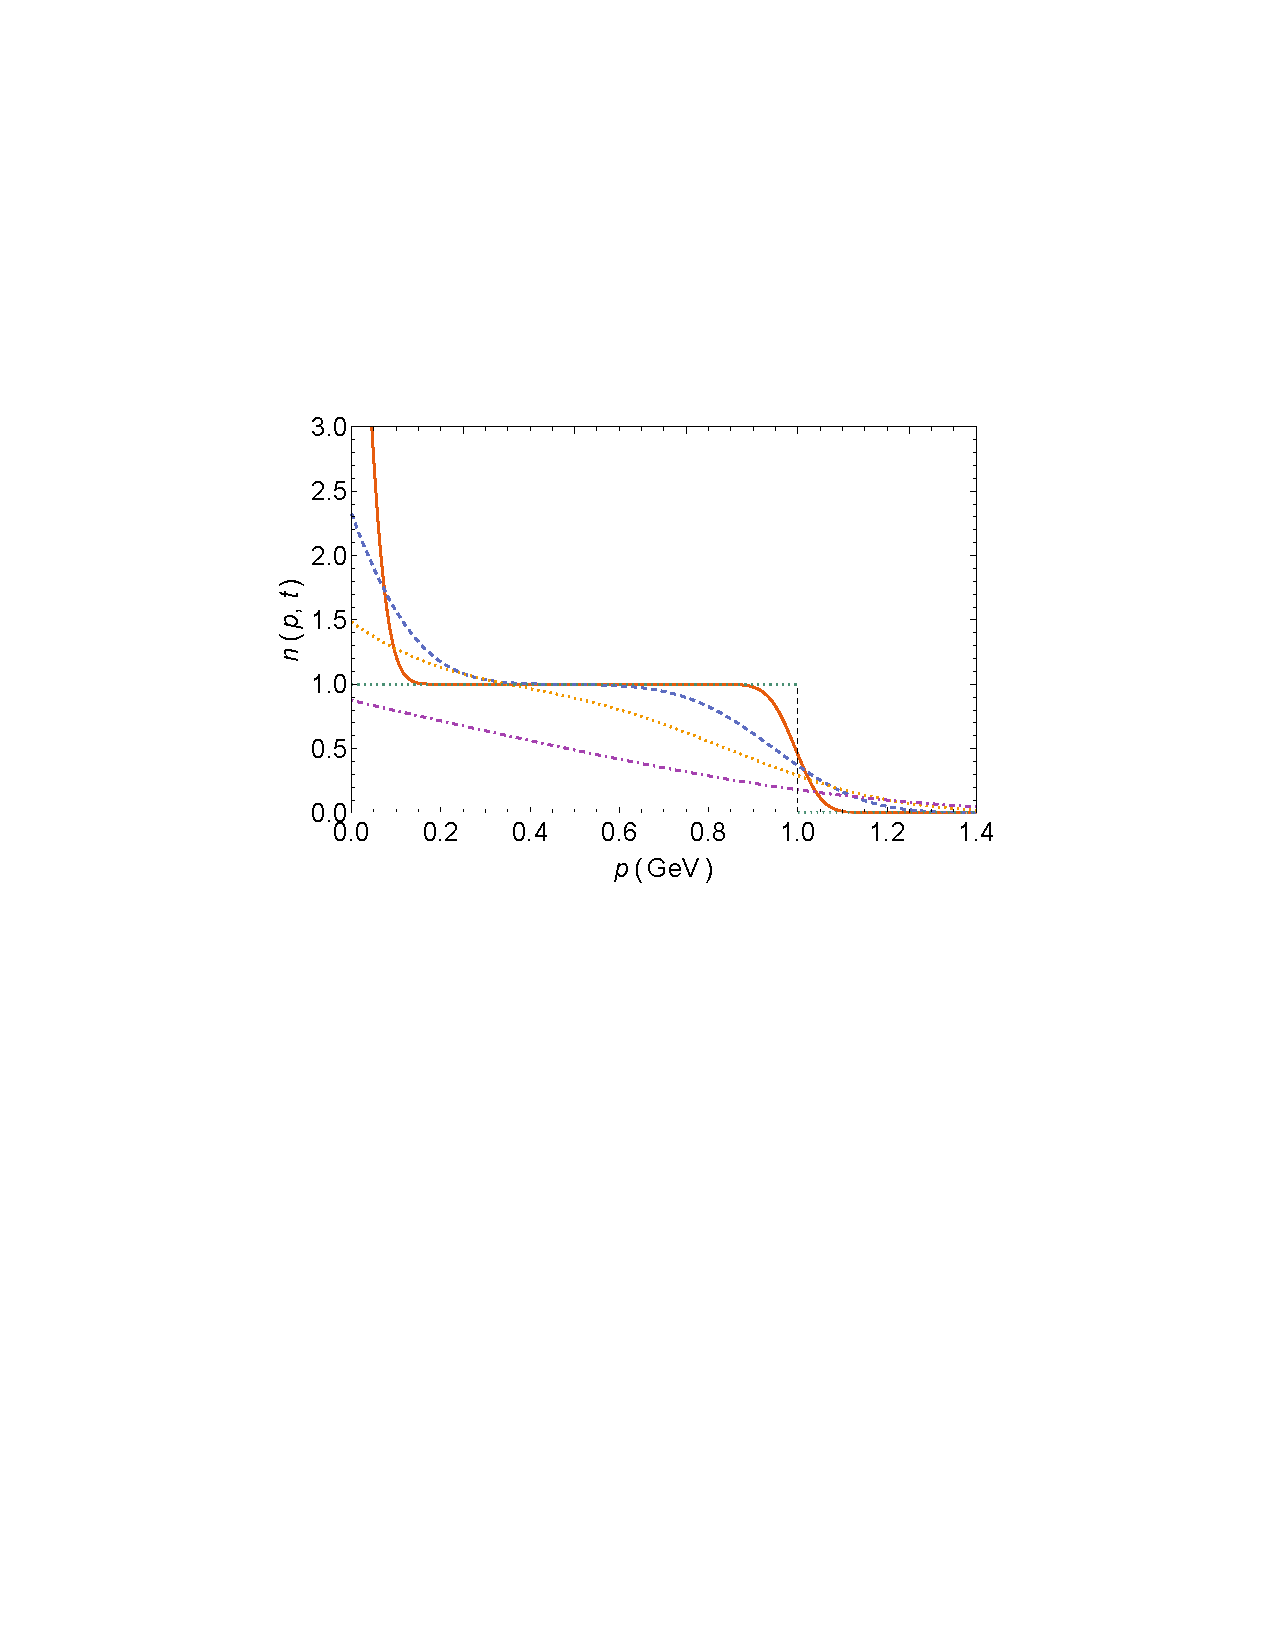
\includegraphics[width=0.8\textwidth]{figures/nbde_positive_range}
\caption{Equilibration of a finite Bose system from the NBDE. \cite{Wolschin2018} \\ 
The integration range is restricted to $x \geq 0$. Here $T\simeq 0.4\ \mathrm{GeV}$, $\tau_{\mathrm{eq}} =  0.33\cdot 10^{-23} \mathrm{s}$ and the timesteps are $\left\{0.005, 0.05, 0.15,0.5\right\}$ (in units of $10^{-23}s$) from top to bottom.}
\end{figure}
\end{frame}

\begin{frame}{Results for the Solution of the NBDE II}
\begin{figure}[H]
\centering
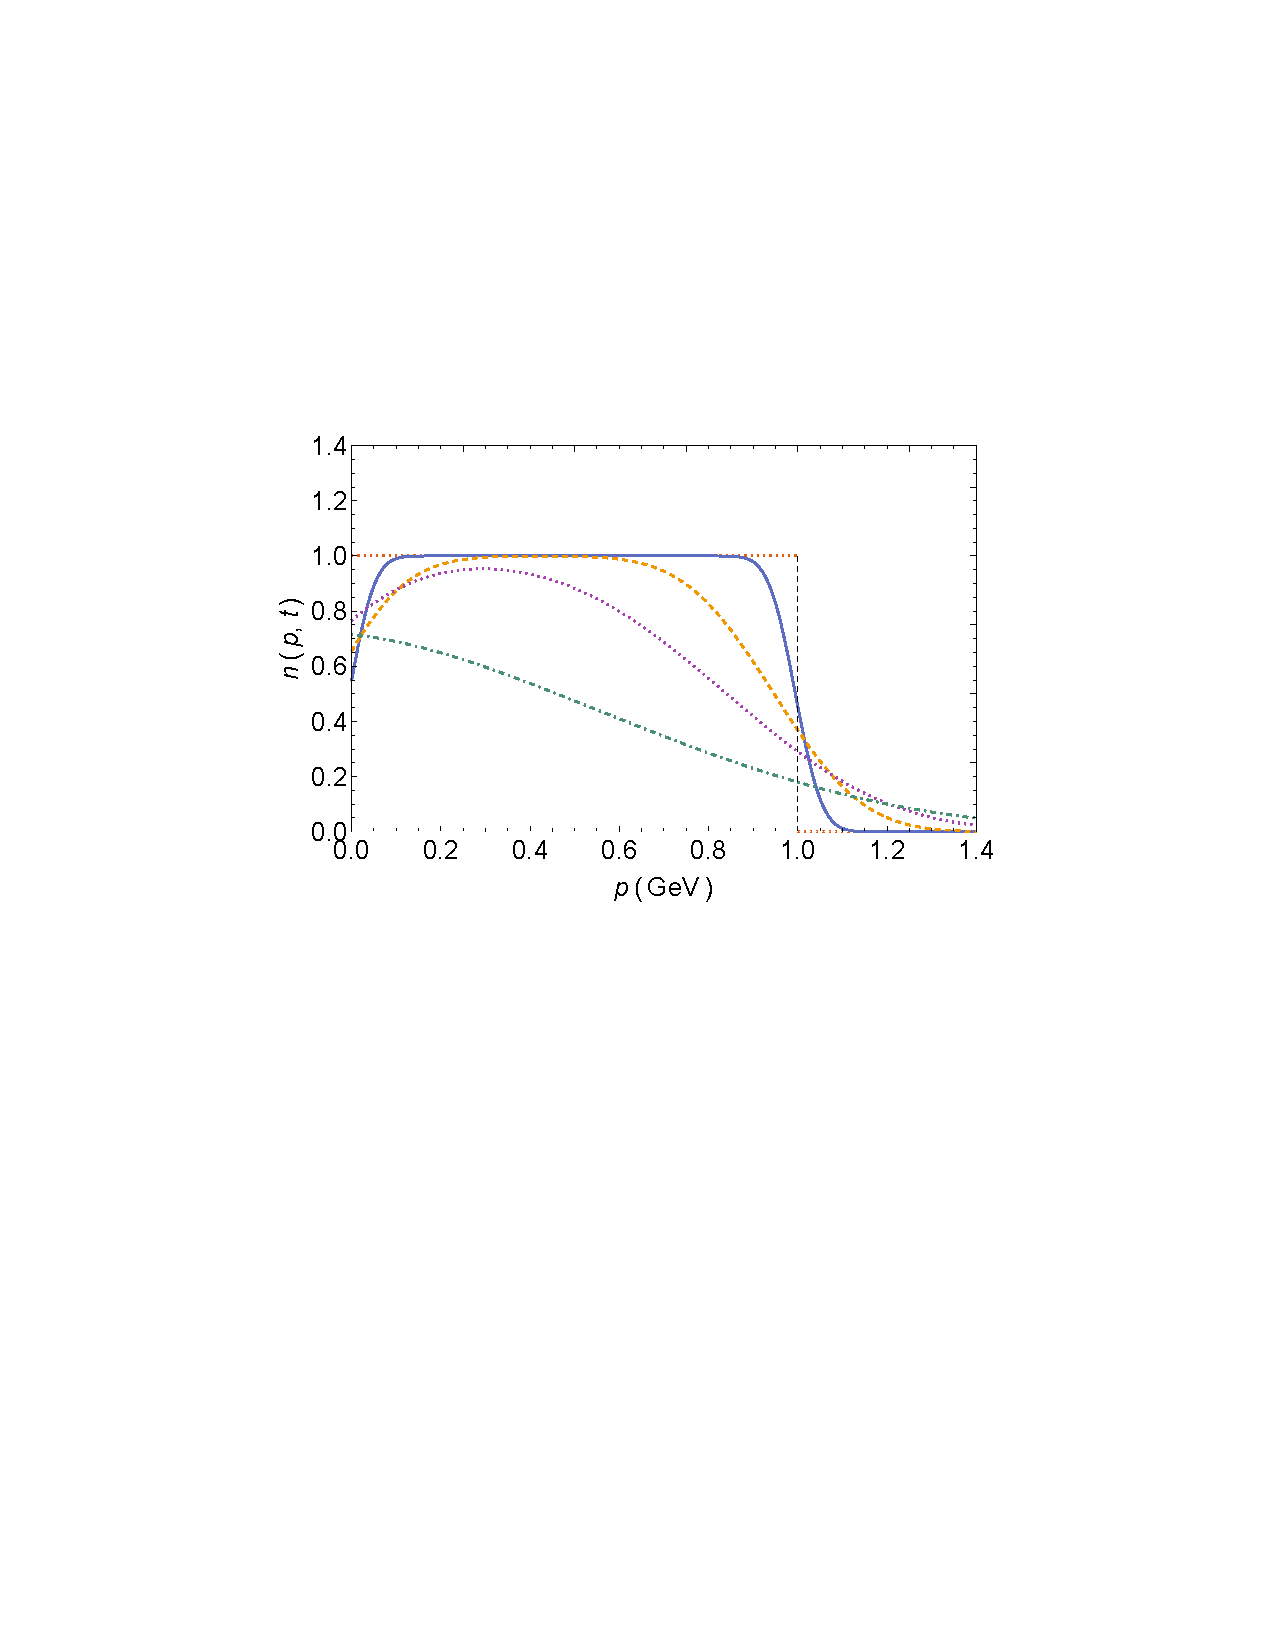
\includegraphics[width=0.8\textwidth]{figures/nbde_full_range}
\caption{Equilibration of a finite Bose system from the NBDE. \cite{Wolschin2018} \\ 
The integration range is extended to $-\infty \leq x \leq \infty$. Here $T\simeq 0.4\ \mathrm{GeV}$, $\tau_{\mathrm{eq}} =  0.33\cdot 10^{-23} \mathrm{s}$ and the timesteps are $\left\{0.005, 0.05, 0.15,0.5\right\}$ (in units of $10^{-23}s$) from top to bottom.}
\end{figure}
\end{frame}


\begin{frame}{Results for the Solution of the NBDE III}
\begin{figure}[H]
\centering
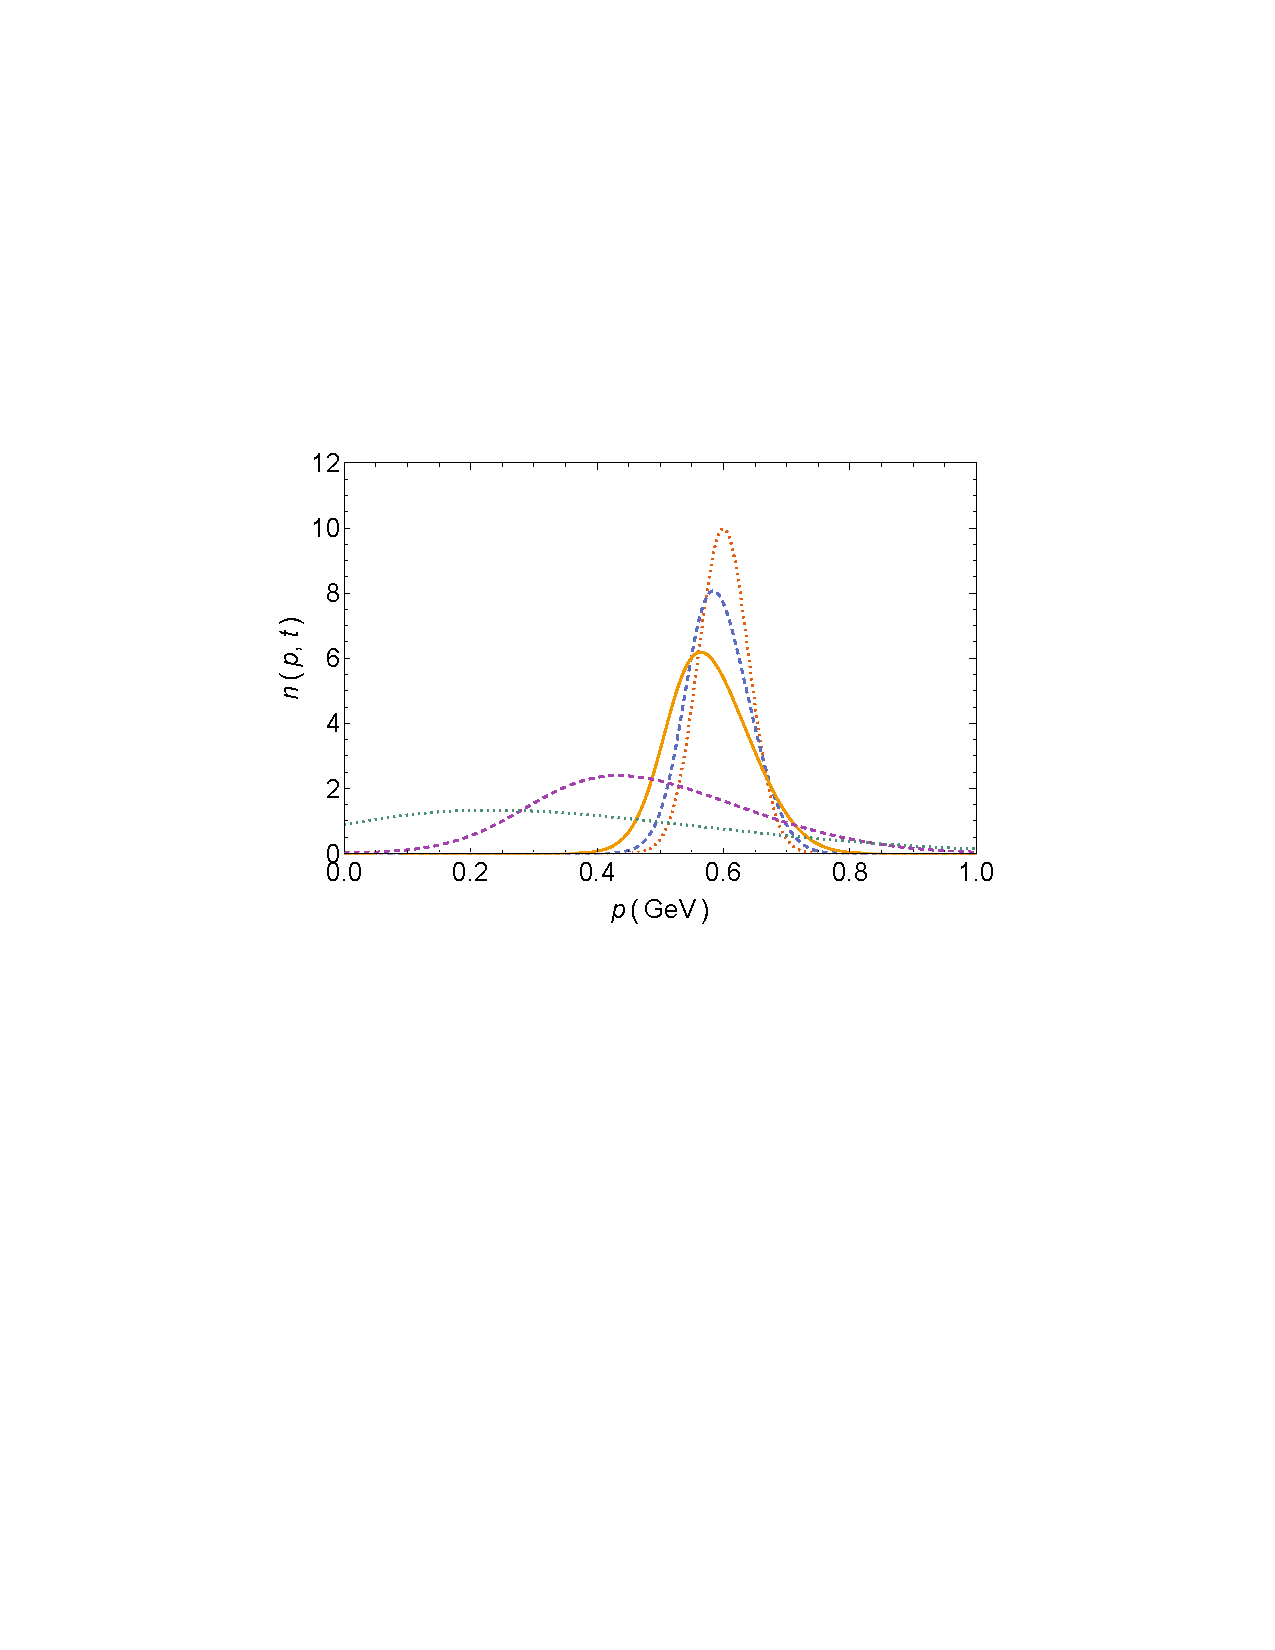
\includegraphics[width=0.8\textwidth]{figures/nbde_gaussian}
\caption{Equilibration of a finite Bose system from the NBDE for Gaussian initial conditions $n_{\mathrm{i}}(\varepsilon) = N_{\mathrm{i}}\left(\sqrt{2\pi}\sigma\right)^{-1}\exp\left((\varepsilon - \langle\varepsilon\rangle)/(2\sigma^2)\right)$ with $\sigma = 0.04\ \mathrm{GeV}$. \cite{Wolschin2018} \\ 
Here $T\simeq 0.4\ \mathrm{GeV}$, $\tau_{\mathrm{eq}} =  0.33\cdot 10^{-23} \mathrm{s}$ and the timesteps are $\left\{0.002, 0.006, 0.02, 0.2\right\}$ (in units of $10^{-23}s$) from top to bottom.}
\end{figure}
\end{frame}



\begin{frame}{Treating the Singularity}
This part is based on the publication \cite{Wolschin2020_1} which provides an extension of \cite{Wolschin2018} and was published just recently.\\[0.5em]	
\begin{itemize}
	\item To account for the singularity at $\varepsilon=\mu < 0$ we have to modify the initial distribution given before (eqn. (\ref{eqn:rta_initial})) as follows:
	\begin{equation}
		\tilde{n_{\mathrm{i}}}(\varepsilon) = n_{\mathrm{i}}(\varepsilon) + \frac{1}{\exp\left(\frac{\varepsilon-\mu}{T}\right)-1}
	\end{equation}
	\item The chemical potential $\mu$ has to be treated as a fixed parameter.
	\item Considering the limit $\lim_{\varepsilon\rightarrow\mu^{+}}\ n(\varepsilon,t) = \infty\ \forall t$ yields $\mathcal{Z}(\mu,t) = 0$.
	\item This results in a modified expression for the Green's function
	\begin{equation}
		G(\varepsilon,x,t) = G_{\mathrm{free}}(\varepsilon-\mu,x,t) - G_{\mathrm{free}}(\varepsilon-\mu,-x,t)
	\end{equation}
\end{itemize} 
\end{frame}

\begin{frame}{Results for the RTA for the modified Initial Conditions}
\begin{figure}[H]
\centering
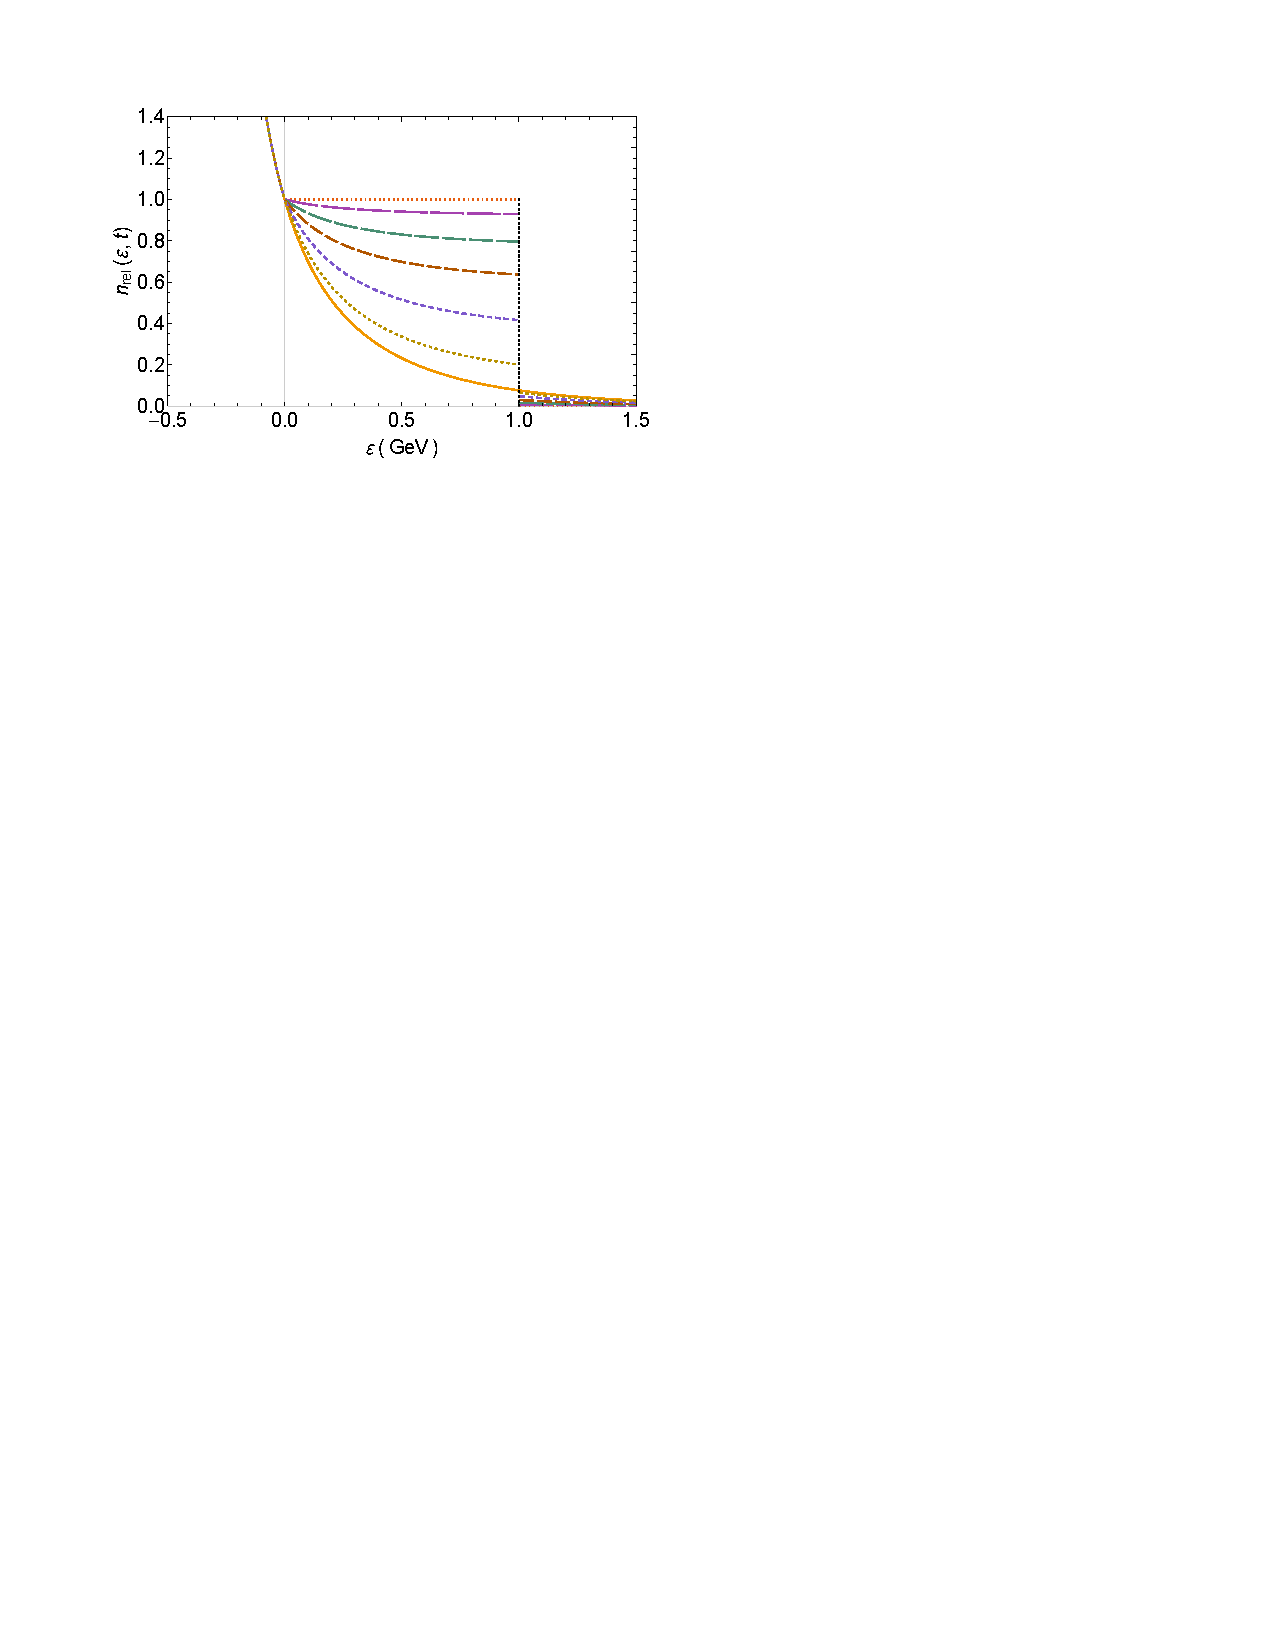
\includegraphics[width=0.8\textwidth]{figures/rta_full}
\caption{Local thermalization of gluons in the linear RTA for $\mu<0$. \cite{Wolschin2020_1} \\ 
Here $T \simeq 513\ \mathrm{MeV}$ and the timesteps are $\left\{0.02, 0.08, 0.15,0.3,0.6\right\}$ (in units of $\mathrm{fm}/c$) from top to bottom.}
\end{figure}
\end{frame}
%TODO: Elaborate on Solutions#2
\begin{frame}{Results for the full Solution of the NBDE}
\begin{figure}[H]
\centering
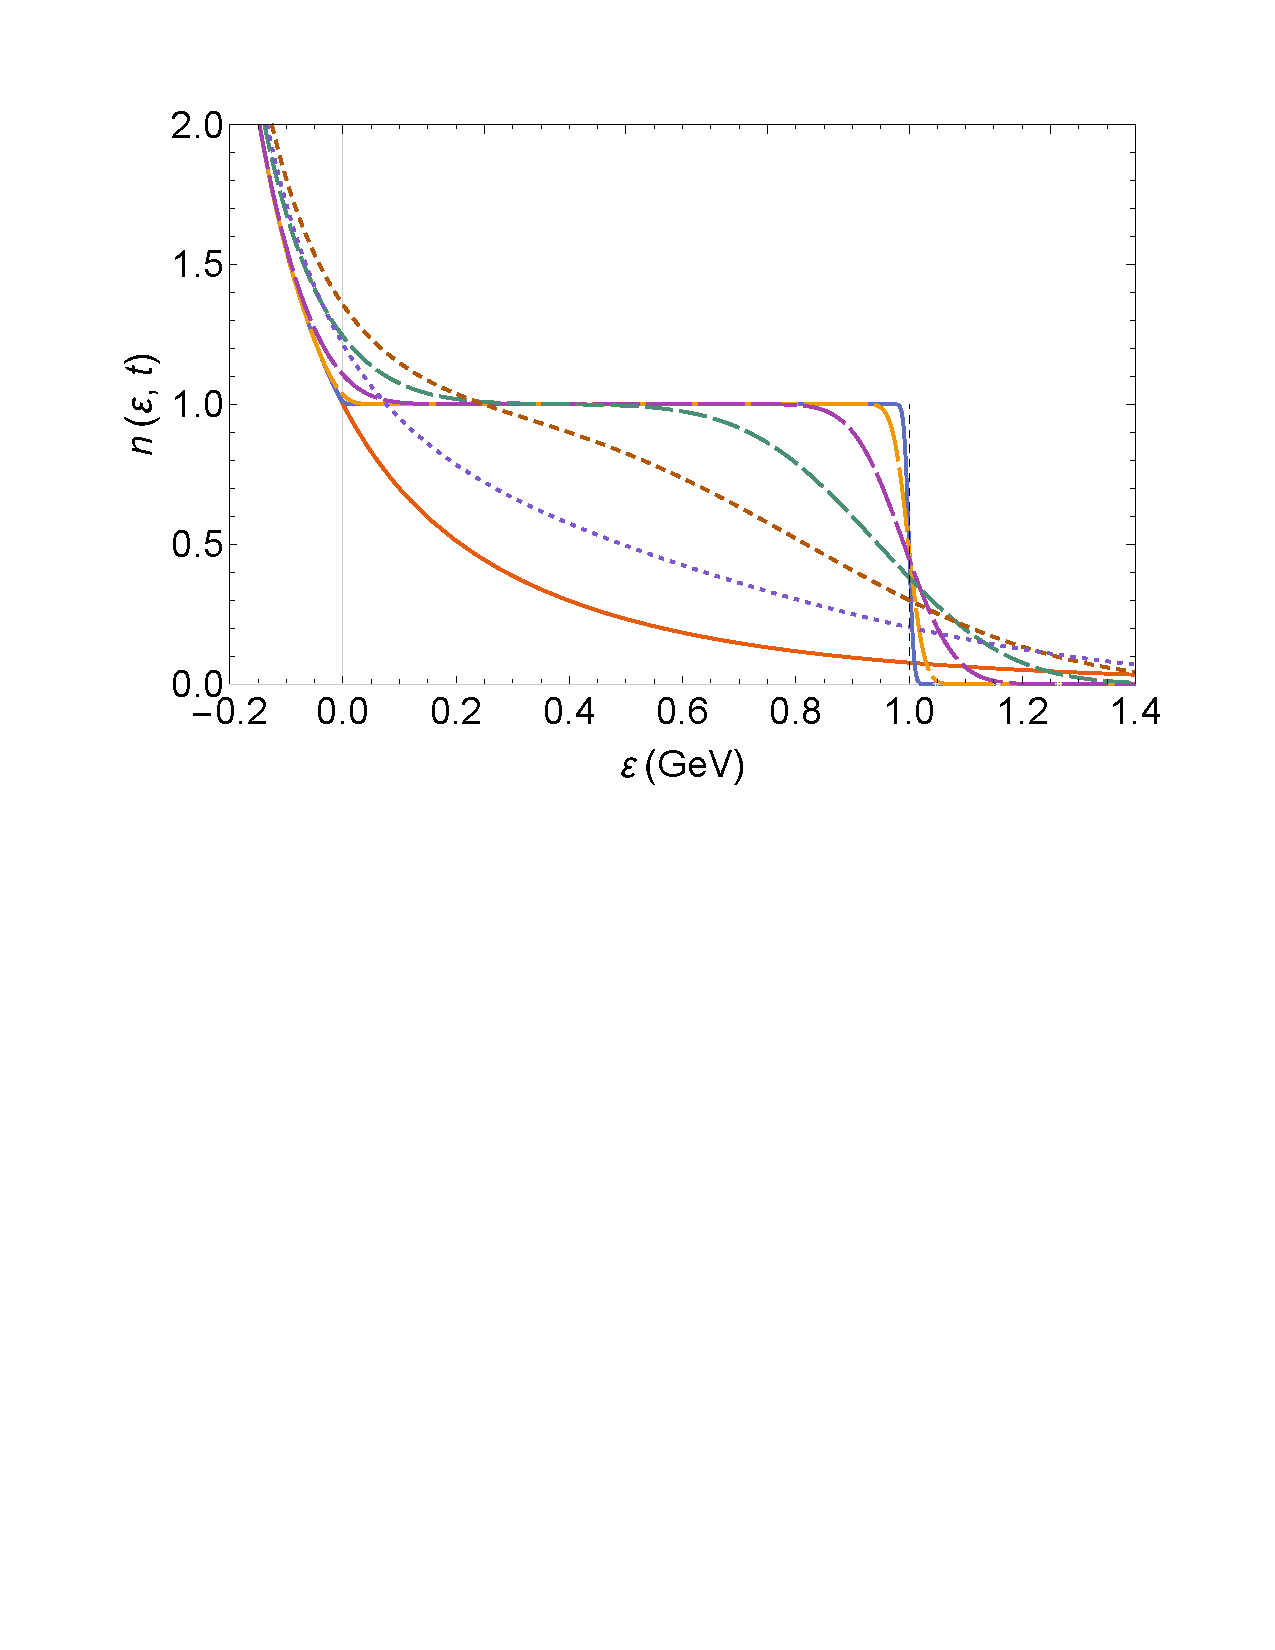
\includegraphics[width=0.8\textwidth]{figures/nbde_full_result}
\caption{Local thermalization of gluons from the time-dependent solutions of the NBDE for $\mu<0$. \cite{Wolschin2020_1} \\ 
Here $T \simeq 513\ \mathrm{MeV}$ and the timesteps are $\left\{6\cdot10^{-5}, 6\cdot10^{-4}, 6\cdot10^{-3},0.12,0.36\right\}$ (in units of $\mathrm{fm}/c$) from top to bottom.}
\end{figure}
\end{frame}